\subsection{Eksportering} \label{sec:Eksport}
Dette afsnit indeholder en gennemgang af den grafiske brugergrænseflade, design og implementering af 'Export viewet' i Rambøll Tilsyn.

\subsubsection{Design}
På Figur \ref{fig:EksporterSekvensDiagram} ses sekvensdiagrammet for 'Export' viewet til Rambøll Tilsyn.
\begin{figure}[H] % (alternativt [H])
	\centering
	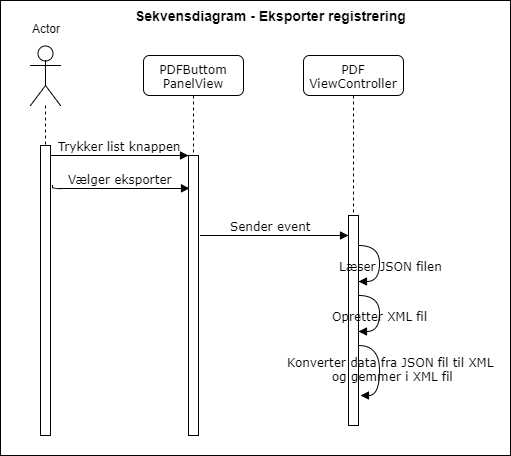
\includegraphics[height=10cm, width=10cm]{../ArkitekturDesign/Design/Eksportering/EksporterSekvensDiagram}
	\caption{Sekvensdiagram for Eksportering i Rambøll Tilsyn.}
	\label{fig:EksporterSekvensDiagram}
\end{figure}

\clearpage

\subsubsection{Grafisk brugergrænseflade}
Efter at have eksporteret registreringen til en XML-fil, vil den se ud som på Figur \ref{fig:Excel}.
\begin{figure}[H] % (alternativt [H])
	\centering
	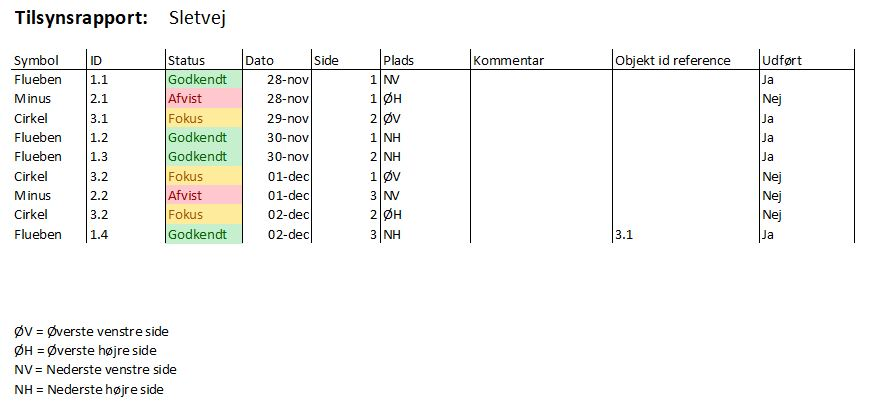
\includegraphics[height=10cm, width=17cm]{../ArkitekturDesign/Design/Eksportering/Excel}
	\caption{Export viewet som det vil se ud, når det er åbent i excel.}
	\label{fig:Excel}
\end{figure}
Tabellen består af linjer, hvor hvert objekt har følgende information: \\
\textbf{Symbol:} Er navnet på den type symbol, som er oprettet. \\
\textbf{ID:} Er objektets id. Dette gives ud fra, hvilken type symbol det er. \\
\textbf{Status:} Viser statussen på objektet. Status følger typen af objekt. \\
\textbf{Dato:} Viser dato for hvornår objektet er oprettet. \\
\textbf{Side:} Viser hvilken side i PDF-tegningen objektet er oprettet på. \\
\textbf{Plads:} Viser hvor på den tilhørende side at objektet er placeret. \\
\textbf{Kommentar:} Giver mulighed for at skrive kommentar til objektet. \\
\textbf{Objekt id reference:} Hvis et objekt bliver ændret fra f.eks. et minus til et flueben, vil der blive oprettet et nyt fluebens objekt, som får reference id til det minus, som er ændret. \\
\textbf{Udført:} Viser om objektet er blevet udført. F.eks. at alle minus og cirkel objekter er blevet ændret til flueben. \\

\subsubsection{Implementering}
Denne funktionalitet er ikke implementeret.

\clearpage